\documentclass[a4paper, varvw, nofootinbib]{revtex4-2}
\usepackage[a4paper,top=1.05in, bottom=0.85in, left=0.85in, right=0.75in]{geometry}
\usepackage[italian]{babel}
\usepackage[utf8]{inputenc}
\usepackage[T1]{fontenc}
\usepackage{microtype}
\usepackage{newtx}
\makeatletter
\let\it@comma@def\active@comma
\makeatother
\usepackage{physics}
\usepackage[round-mode = uncertainty]{siunitx}
\usepackage{graphicx}
\usepackage[hidelinks]{hyperref}

\def\bibsection{\section*{\refname}}

\begin{document}
\title{Determinazione della carica elementare, della costante di Plank e della costante di Boltzmann}
\author{Andrea Parodi}
\author{Francesco Polleri}
\author{Mattia Sotgia}
\email{s4942225@studenti.unige.it}
\affiliation{Dipartimento di Fisica, Università degli Studi di Genova, Genova, Italia}
\date{7 dicembre 2022}

\begin{abstract}
Presentiamo la misura dei valori della carica dell'elettrone $e$, della costante di Planck $h$ e della costante di Boltzmann $k$ come combinazione di quattro esperimenti separati ed indipendenti, mirati alla misura dei rapporti $e/h$, $e/k$ \cite{inmanMeasurementIntroductoryPhysics1973} e $h/k$, insieme all'esperimento proposto da Millikan \cite{millikanIsolationIonPrecision1911} per ottenere un valore della carica elementare $e$. Ci concentriamo sulla misura del rapporto $h/k$ realizzando lo stesso esperimento proposto in \cite{crandallMinimalApparatusDetermination1983}, sfruttando quindi la radiazione di corpo nero in una sua applicazione realizzabile in laboratorio. Combiniamo quindi i risultati in uno studio statistico ottenendo un valore preciso per le costanti $h$, $e$, $k$.
\end{abstract}

\maketitle

\subparagraph*{Introduzione} Vogliamo ottenere una misura precisa del valore della carica dell'elettrone $e$, della costante di Planck $h$ e della costante di Boltzmann $k$. Per ottenere la misura di queste tre costanti ci concentriamo sulla realizzazione di quattro esperimenti, separati ed indipendenti. Non è facile infatti, eccetto per il caso della carica elementare, realizzare un singolo esperimento che permetta di misurare il valore di $h$, $k$ in modo diretto, ma sono invece realizzabili alcuni esperimenti che permettono di ottenere il valore dei rapporti a coppie di queste tre quantità \cite{inmanMeasurementIntroductoryPhysics1973, millikanIsolationIonPrecision1911, crandallMinimalApparatusDetermination1983}. Otterremo infatti la misura del rapporto $e/h$ studiando la curva di risposta del passaggio di corrente attraverso una giunzione \emph{p-n}, come un {LED}, rispetto alla tensione fornita in alimentazione. La misura di $e/k$ è invece ottenuta in modo simile, però studiando la risposta di un transistor ad un segnale di tensione in ingresso. Infine a partire dalla legge di Boltzmann, sfruttando la legge della radiazione di corpo nero di Planck andiamo a calcolare il valore di $h/k$. 

Ai tre esperimenti realizzati in laboratorio sono poi aggiunti dati di misurazioni dell'esperimento di Millikan che permettono di ottenere una stima di $e$. Dati quindi i quattro valori ottenuti possiamo ottenere una miglior stima delle costanti fisiche realizzando una analisi statistica.

\paragraph*{Risposta in corrente di una giunzione \emph{p-n}, misura di $e/k$}

È noto per le conclusioni tratte già da \cite{einsteinConcerningHeuristicPoint1965} e poi dai risultati della meccanica quantistica che una particella, carica elettricamente, se colpita con sufficiente energia $E$ produce un fotone di frequenza $\nu$ e una particella identica ma di energia inferiore. La relazione che lega $E$ e $\nu$ è data da $E=h\nu$, e la costante di proporzionalità è la costante di Planck. Non è però facile misurare in modo diretto il valore dell'energia per poter ricavare una stima immediata di tale costante. In un diodo, ovvero un elemento circuitale costituito da due giunzioni semiconduttrici drogate in modo diverso, avremo che il passaggio di corrente avviene quando gli elettroni della giunzione $n$ sono spinti a uscire dalle loro orbite stabili e andare a rimediare alla mancanza di cariche negative della giunzione $p$. Quando questo passaggio avviene gli elettroni rilasciano energia, in forma quantizzata, come fotoni di luce. Nei led il drogaggio \emph{p-n} è tale per cui l'energia rilasciata $E$ corrisponde una frequenza $\nu$ nel visibile. L'energia che viene rilasciata è pari al lavoro che viene compiuto per spostare gli elettroni, che in termini della tensione si traduce in un lavoro $\mathcal W = e V_\text{diode}$, che permette di stabilire una relazione lineare $h\nu = eV_\text{diode}$ per cui trovato il valore di tensione per cui si attiva il LED, si può ottenere una stima di $e/h$.

\paragraph*{Risposta in tensione di un transistor, misura di $e/h$}

Come i LED anche i transistor sfruttano giunzioni \emph{p-n} di semiconduttori. Quando una giunzione \emph{p-n} viene creata, la corrente che si instaura è esponenzialmente proporzionale alla tensione, $I=A\exp(-eV_0/kT)$, con un coefficiente che permette di trovare una stima di $e/k$. Però la relazione in condizioni reali deve essere corretta, dotandosi di un coefficiente $\eta$ che varia per ogni diodo. Stabilità maggiore è però ottenuta considerando una giunzione tripla \emph{n-p-n}, mantenendo la prima e l'ultima giunzione, ovvero emettitore e collettore, allo stesso potenziale. In questo caso la corrente elettrica è descritta come \begin{equation} I = I_0 \qty(\exp(\frac{eV_{t}}{kT}) - 1). \end{equation}

\paragraph*{Radiazione di corpo nero} Per un corpo nero è valida la relazione trovata da Planck per cui l'intensità di radiazione emessa ha una dipendenza dalla temperatura descritta dalla relazione \begin{equation} \mathcal I(\nu, T) = \frac{8 \pi h \nu^3}{c^2}\qty(\exp(\frac{h\nu}{kT})-1)^{-1}.  \end{equation} Selezionando una sola frequenza di radiazione $\nu$, allora avremo che dividendo membro a membro otteniamo una relazione più agevole, e siccome per frequenze ottiche ($\SI{350}{\nano\metre} < \nu <\SI{700}{\nano\metre}$) abbiamo che $h\nu \ll kT$, ovvero che l'esponenziale si sviluppa intorno allo zero, potendo semplificare la relazione precedente. Avremo che allora la relazione semplifica come \begin{equation} \log(\frac{\mathcal I_j}{\mathcal I_i}) = \frac{h\nu}{k}\qty({1\over T_i} - {1\over T_j}),~\text{ dove $h/k$ è considerato parametro di fit.} \label{eq:3}\end{equation}

In una prima approssimazione una lampadina alogena può essere considerata essere un esempio di corpo nero, per cui il bilancio di potenza fornisce $P_\text{abs} + P_e = P_\text{em} + P_\text{cond}$, dove $P_\text{amb} = AT_\text{amb}^4$ è la potenza assorbita dall'ambiente, che consideriamo trascurabile, come anche $P_\text{cond}$ che è legata alla conduzione elettrica. 
Vogliamo ora osservare eventuale dipendenza della temperatura di emissione dalla temperatura ambiente per il setup considerato. Da prima avremo che $P = AT^4$.  Allora assumendo una dipendenza della temperatura dalla resistenza come $T = \beta R^\gamma$, possiamo anche ottenere una dipendenza della dispersione in ambiente, per cui $P_\text{amb} = AT_\text{amb}^4 = \beta A R^{4\gamma}_\text{amb}$, e per la potenza emessa dal corpo nero, per cui $P = AT^4 = \beta A R^{4\gamma}$. Dividendo membro a membro avremo allora la dipendenza della temperatura dalla temperatura ambiente, e sostituendo per la potenza emessa avremo allora \begin{equation} P = VI =  A \qty[\qty(\frac{V}{IR_\text{amb}})^\gamma T_\text{amb}]^4.\label{eq:4} \end{equation} 

\subparagraph*{Metodi}\label{sec:black_body_methods} Il setup sperimentale piuttosto semplificato prevede una lampada alogena che emette radiazione non polarizzata su uno spettro ampio. Di questo spettro si considera un taglio preciso con un filtro ottico che permette di avere $\nu = \SI{6.66(6)e+5}{\giga\hertz}$, dovuta ad una lunghezza d'onda $\lambda \simeq \SI{450}{\nano\metre}$. L'intensità luminosa viene poi quantificata utilizzando un fotodiodo per il quale $V_\text{fd} \propto \mathcal I_\text{fd}$, per cui la relazione \eqref{eq:3} allora si ottiene nella forma \begin{equation}\underbrace{\log(\frac{V^\text{fd}_j}{V^\text{fd}_i})}_{(\text{LOG})_i^j} = \frac{h}{k}\underbrace{\nu\qty({1\over T_i} - {1\over T_j})}_{{\Delta_{\frac{1}{T}}}_i^j}. \label{eq:5}\end{equation}

\begin{figure}
    \centering
    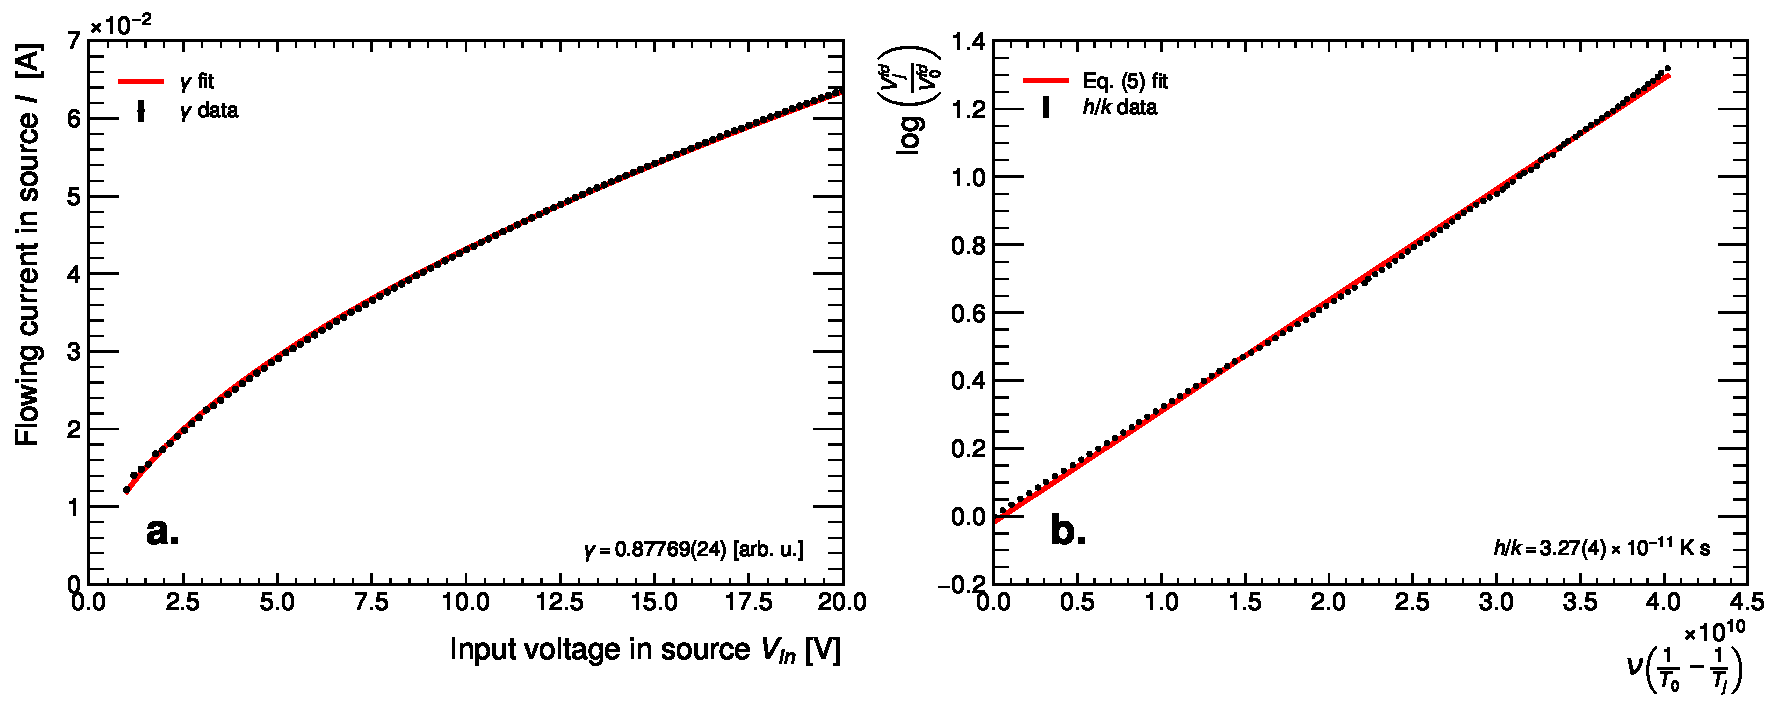
\includegraphics[width=14cm]{fig/plot_hk}
    \caption{\textbf{a.} Considerati coppie di punti in tensione e corrente, possiamo caratterizzare il circuito della sorgente e la sua risposta in termini di temperatura, ovvero ottenere il valore di $\gamma$. \textbf{b.} I dati raccolti e trasformati secondo la relazione \eqref{eq:5} cono fittati su un set di dati considerato $j=0$.}
\end{figure}

\paragraph*{Misura della dipendenza da $\gamma$ per la temperatura} Caratterizziamo l'apparato sulla base della relazione \eqref{eq:4}, ovvero otteniamo un valore di $\gamma$ per cui la relazione è valida. Ipotizzando la temperatura ambiente costante, avremo che a meno di costanti la relazione \eqref{eq:4} ci permette di avere una stima di $\gamma$. Troviamo allora che \[\gamma = \num{0.87769(24)}.\] Noto quindi il valore di $\gamma$ è possibile determinare la temperatura della sorgente in dipendenza dalla tensione fornita e alla corrente che circola sul circuito. La temperatura risulterà essere allora una funzione $T_j = T_j(V_j, I_j, \gamma)$, oltre che dipendente dalla temperatura ambiente $T_\text{amb}$, misurata indipendentemente durante la presa dati, $T_\text{amb} = \SI{299.7 +- 0.7}{\kelvin}$, e dall'impedenza a temperatura ambiente $R_\text{amb} = \SI{25.045 +- 0.215}{\ohm}$ misurata a priori della presa dati. Osserviamo dunque che quindi i diversi valori di temperatura $T_j$ risulteranno essere tra loro correlati. 

\paragraph*{Calcolo del rapporto $h/k$} La relazione \eqref{eq:5} è una relazione che permette facilmente di ottenere una buona stima del rapporto $h/k$, a patto di tenere in considerazione tutte le possibili correlazioni che naturalmente intervengono nel passaggio dal set di dati $(V_j^\text{fd}, T_j)$ alla forma $((\text{LOG})_i^j, ({\Delta_{\frac{1}{T}}}_i^j))$ dove queste ultime notazioni indicano i due membri della relazione lineare espressa in \eqref{eq:5}. Possiamo però ipotizzare di non considerare gli errori sulle temperature, e associare alla funzione $(\text{LOG})_i^j$ solo l'errore legato al valore di $V_j^\text{fd}$. 
Inoltre, dopo aver appurato che il metodo e il risultato non dipendano da tale scelta, possiamo da ora in poi utilizzare la convenzione per cui nella relazione \eqref{eq:5} il valore di $i=0$. Avremo che allora si potrà eseguire un fit con le variabili $(\text{LOG})_0^j\pm\sigma_\text{LOG$_0^j$}$ e ${\Delta_{\frac{1}{T}}}_0^j$. A questo punto, facendo variare individualmente ogni valore che determina il fit della funzione consideriamo lo scarto legato ad ognuna variazione individuale, e, dopo aver verificato che in questo modo lo scarto sia inferiore percentualmente all'errore percentuale del fit iniziale, procediamo a sommare in quadratura tutti i contributi, fino ad ottenere il valore della deviazione standard associata alla miglior stima di $h/k$. Otteniamo allora \[h/k = \SI{3.27(4)e-11}{\kelvin\second}.\]

\begin{figure}
\centering
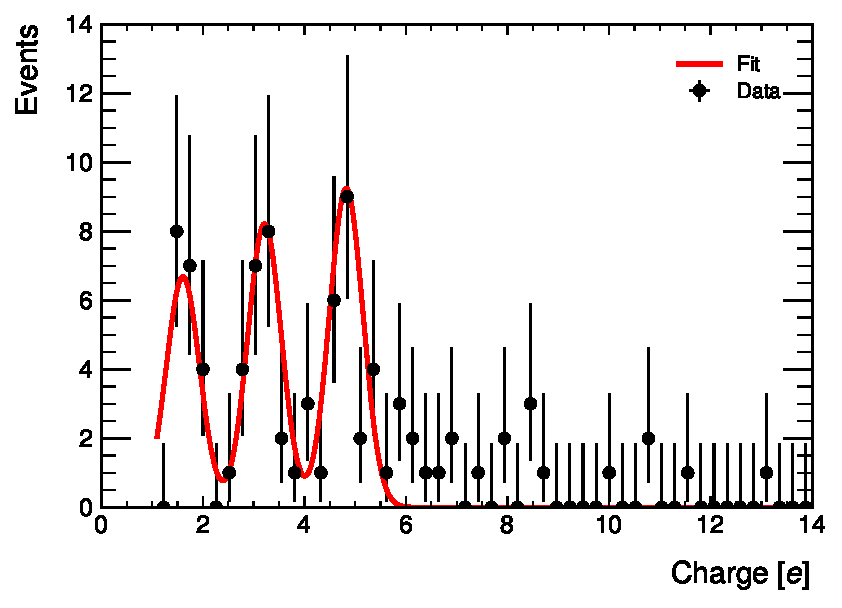
\includegraphics[width=14cm]{fig/millikan}
\caption{Minimizzazione della Eq. \eqref{eq:6} con \emph{maximum Likelihood (MLE)} per ottenere una stima dei parametri della distribuzione di probabilità $f_\text{Mlk}$. Il parametro principale che interessa ottenere è però il valore di separazione tra i centri delle distribuzioni gaussiane, che corrisponde alla carica dell'elettrone $e$.}
\end{figure}

\subparagraph*{Determinazione indipendente della carica elementare}\label{sec:millikan} Utilizzando un set di dati dall'esperimento di Millikan vogliamo ottenere una stima indipendente della carica elementare $e$. L'esperimento ci permette di avere il valore della carica elementare sfruttando proprio il fenomeno della quantizzazione. Infatti una differenza di potenziale si pone in equilibrio con la forza gravitazionale, permettendo di conoscere la carica depositata su gocce d'olio. Queste si posizioneranno a distanza proporzionale alla carica elementare. I dati raccolti saranno adattabili a più gaussiane, separate ciascuna da un delta $\propto e$. La forma della distribuzione di probabilità sarà quindi trovata come \begin{equation} f_\text{Mlk} =  A_0 \frac{1}{\sqrt{2\pi\sigma^2}}\exp({-\frac{e}{2\sigma^2}}) +  A_1 \frac{1}{\sqrt{2\pi\sigma^2}}\exp({-\frac{2e}{2\sigma^2}}) + (1-A_0-A_1) \frac{1}{\sqrt{2\pi\sigma^2}}\exp({-\frac{3e}{2\sigma^2}}), \label{eq:6}\end{equation} dove i fattori $A_0$, $A_1$ e $1-A_0-A_1$ sono necessari per rendere di norma unitaria la distribuzione. Eseguendo una massimizzazione \emph{binned} della Likelihood (minimizziamo $-\log \mathcal L(f_\text{Mlk})$) otteniamo allora la stima della carica elementare \[e = \SI{1.608(20)e-19}{\coulomb}.\] 

\subparagraph*{Calcolo delle costanti $e$, $h$, $k$ e conclusioni}\label{sec:combined_data} 

\bibliography{ref/ref1}

\end{document}
